\documentclass[11pt]{article}
\usepackage{hyperref}
\usepackage[english]{babel}
\usepackage{blindtext}
\usepackage{url}
\usepackage{graphicx}
\usepackage{multicol}
\usepackage{geometry}
\usepackage[sort, numbers]{natbib}

\usepackage{fancyhdr}


\graphicspath{ {/home/joebrew/Documents/uf/phc6016/loi} }


\usepackage{Sweave}
\begin{document}
\Sconcordance{concordance:loi.tex:loi.Rnw:%
1 20 1 1 0 84 1 1 43 1 2 4 1 1 13 1 2 10 1}


\newgeometry{margin=1.5cm}
\fancyhfoffset[E,O]{0pt}

%------------------------------------------
\section*{Childhood obesity: social import of place}
%------------------------------------------
Joe Brew 

\noindent \hrulefill


%------------------------------------------
\subsection*{Introduction}
%------------------------------------------
The prevalence of obesity among American school-aged children has grown in recent decades at an alarming rate (figure 1)\cite{Ogden2014}. Obesity has a steep social gradient, and areas that are poor or socially marginalized have above average rates in the USA.\cite{Budd2014} Because obesity is closely correlated with socieconomic status, which is in turn associated with residential location, studying geography's independent association with childhood obesity is extremely challenging. 

Alachua County, Florida, offers the ideal location for the study of childhood adiposity and geography.  

%------------------------------------------
\subsection*{Aims}
%------------------------------------------


%------------------------------------------
\subsection*{Statement of need}
%------------------------------------------


%------------------------------------------
\subsection*{Methodology}
%------------------------------------------


%------------------------------------------
\subsection*{Conclusion}
%------------------------------------------


%----------------------------------------------------------------------------------------
\subsection*{Figures}
%----------------------------------------------------------------------------------------
\begin{center}
Figure 1: Obesity among American children\cite{NIH}
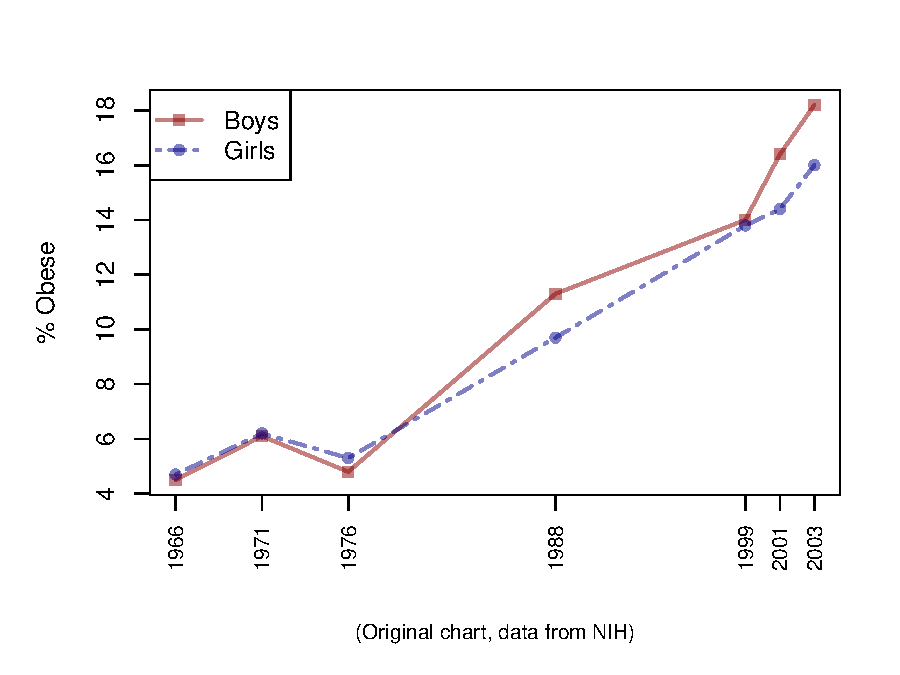
\includegraphics{loi-001}
\end{center}

%----------------------------------------------------------------------------------------
%  REFERENCE LIST
%----------------------------------------------------------------------------------------
\newpage
\bibliographystyle{unsrtnat}
\bibliography{test}




\end{document}
